\section{Background and Related work}

\subsection{Previous work}
It has been only a few years since deep learning frameworks were introduced to public.
Few attempts recently tried to benchmark and compare the performance of the frameworks.
A benchmark of CNN frameworks is publicly available on Github\cite{convnet-benchmarks}.
It shows forward and backward propagation time of CNN model for each framework.
But the latest result was tested with cuDNN version R4, while the most recent version is R5.1.
Detailed benchmarks of deep learning frameworks were recently published\cite{DBLP:journals/corr/BahrampourRSS15, DBLP:journals/corr/ShiWXC16}.
They show execution times of various DNN models run on the frameworks.
However, the benchmarks show only the results, without identifying the reasons for the differences.
They also use cuDNN version of R4, which do not support most recent Winograd convolution.


\subsection{Machine learning frameworks}

Theano is a python framework for evaluating mathematical expressions\cite{DBLP:journals/corr/Al-RfouAAa16}.
It is one of the earliest framework used to build DNN models.
Multiple machine learning frameworks are built on top of Theano.
Pylearn2, Keras and Lasagne are popular frameworks for DNN using Theano as their backend.
Multiple GPU support of Theano is still on experimental stage.
Torch is a scientific computing framework based on LuaJIT\cite{torch}.
Torch is also one of the earliest frameworks used to implement CNN models.
Nvidia's self-driving car project and Deepmind's Deep Q Learning model were built on Torch\cite{nvdave, mnih2015humanlevel}.
Torch natively supports multi-gpu context via its cutorch module.
Caffe is deep learning framework developed by Berkeley Vision and Learning Center\cite{jia2014caffe}.
Caffe use prototxt file to describe DNN models.
Pre-trained network models can be imported with prototxt files.
Visual recognition challenge winners are usually implemented by Caffe\cite{ILSVRC15, RCNN, vgg}.
The flexibility of Caffe is limited.
Introducing a new feature to a layer requires re-building of the entire source code.
The multi-gpu support of Caffe is limited to batch data parallelism.
Tensorflow is machine learning framework developed by Google\cite{tensorflow2015-whitepaper}.
It was first introduced to public in 2015, and is now the most popular machine learning framework on GitHub.
Tensorflow supports both Python and C++ interface.
Computational Network Toolkit(CNTK) is deep learning framework developed by Microsoft\cite{cntk}.
CNTK supports both Windows and Linux environment, while the others do not support Windows.
CNTK uses its own BrainScript to describe DNN models.
It also supports C++ and C\# wrappers to evaluate models.

\begin{figure}
  \centering
  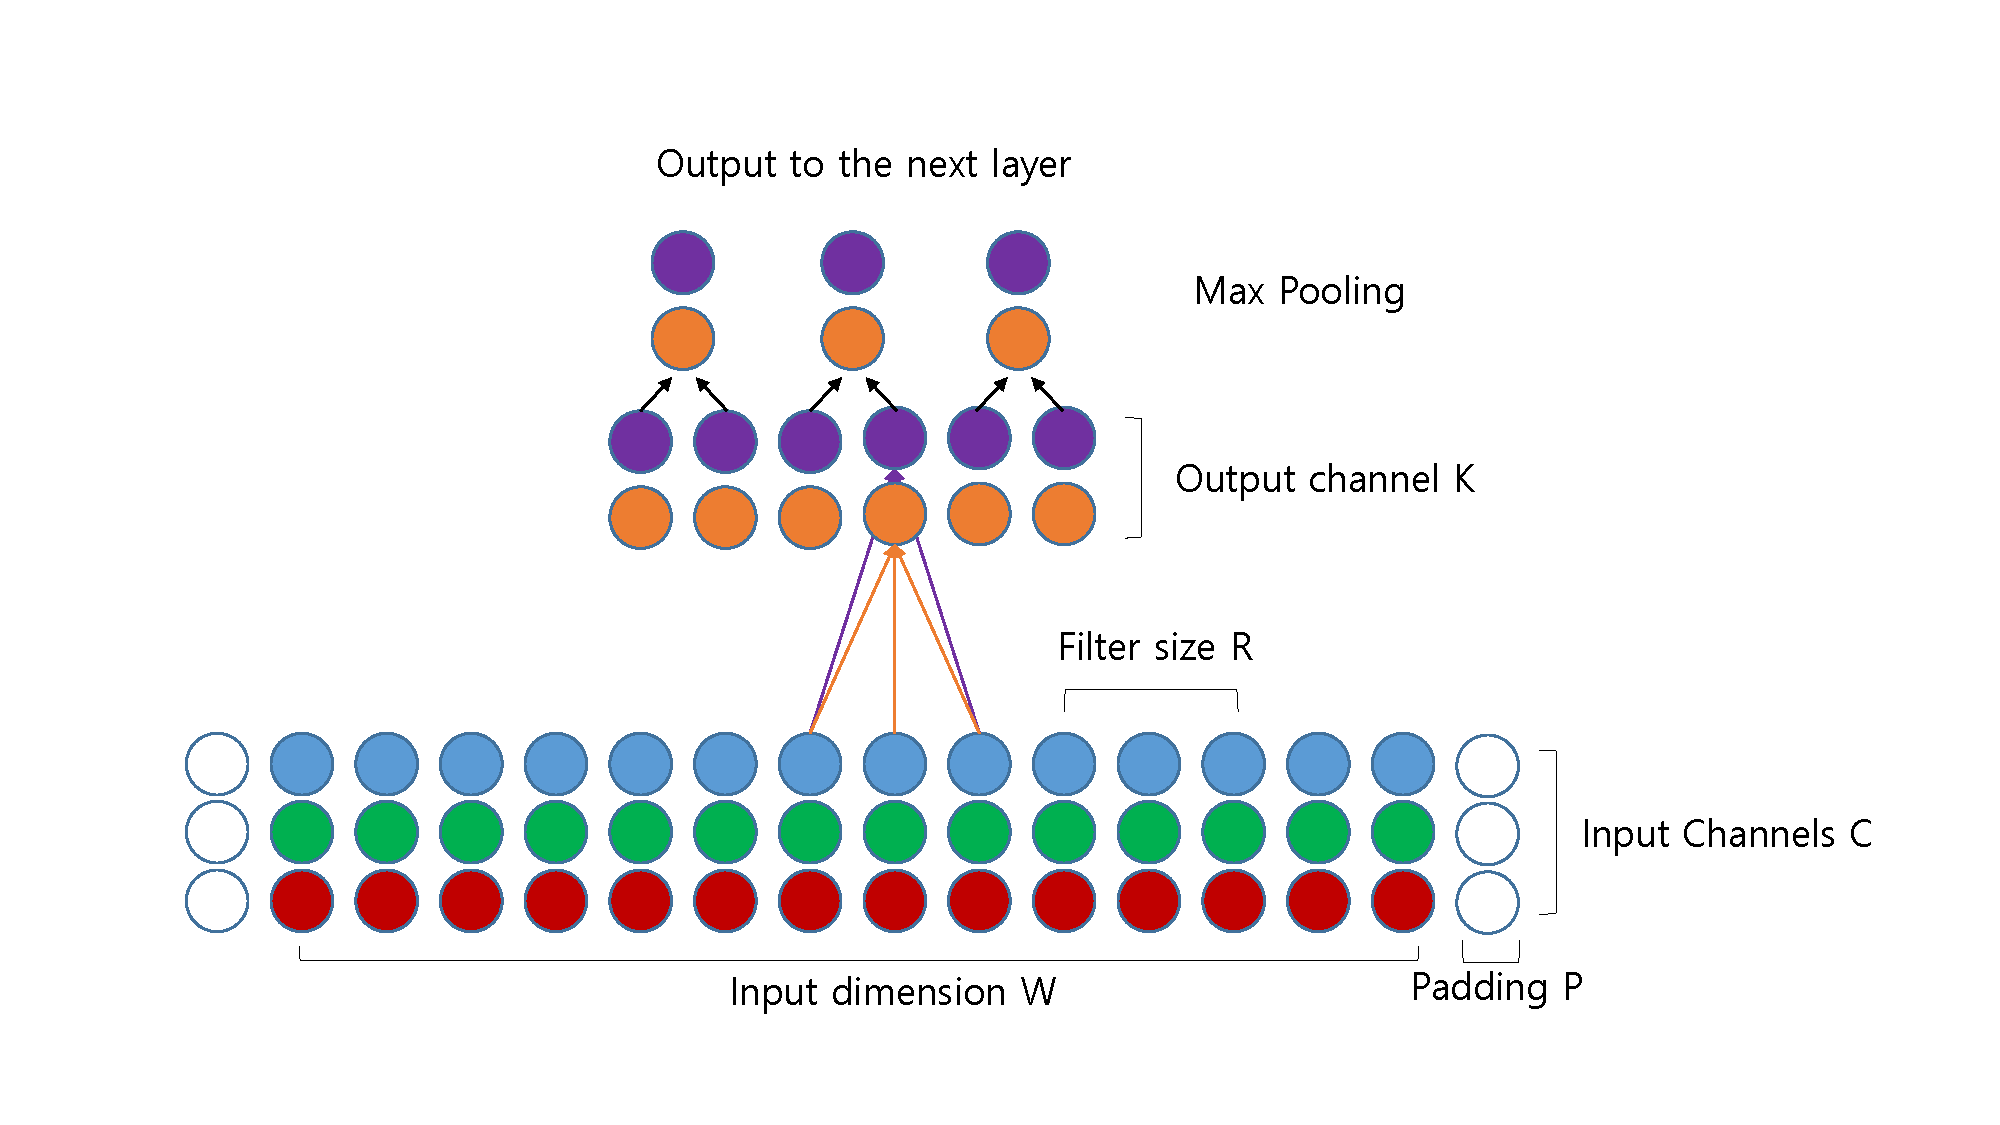
\includegraphics[width=\linewidth]{./figures/convlayer}
  \caption{An example of typical 1D convolution. K filters of filter size R convolves among input of dimension W with C channels.
	Each convolutional filter becomes an output channel. Pooled output feature map is fed to the next layer. }
  \label{fig_convlayer}
\end{figure}

\subsection{Convolutional Neural Network}
Convolutional Neural Network(CNN) is an Artificial Neural Network using convolutional filter to extract features from input.
Figure \ref{fig_convlayer} shows an example of 1D convolutional layer.
K filters of filter size R convolves among input data of dimension W.
Each convolutional filter activation corresponds to a channel of output feature map.
A nonlinear activation function is applied to calculate an activation of a filter.
Typical CNN uses Rectified Linear Unit(ReLU) for nonlinear activation.
A convolution by stride S and padding P creates a feature map of dimension (W - R + P + 1)/S with K channels.
Usually a pooling layer is applied to reduce the output dimension.
The convolutional layer can be extended to multi-dimensional data using tesor data structures.
For example, typical input data for 2D spatial convolution is formatted as 4D tensor of <batch, channel, height, width>(NCHW).
The convolution filters are formatted as <kernels, height, width>(KRS), convolving along each axis.
The computational complexity of propagating such convolutional layer is O(K * CRS * NHW).

\subsection{Convolution algorithms}
Several methods are used to efficiently implement convolution on GPU.
Direct convolution is the most straightforward way but needs a lot of specialized kernels to optimize for various input dimensions and corner cases.
Cuda-convnet \cite{cuda-convnet} is the efficient direct convolution library written by Alex Krizhevsky, the author of AlexNet paper.
CuDNN however, treats convolution as matrix multiplication(GEMM) \cite{cudnn}.
The convolution layer of K kernels with dimension R*R and W*W input with C channels is converted to multiplication of K*CRR filter matrix and CRR*NWW data matrix.
The dimensions of matrices are very big, hence the multiplication can be parallelized using highly efficient BLAS libraries.
Converting convolution to matrix might require significant amount of memory bandwidth.
CuDNN computes the multiplication by tiles to hide memory latency while computing.
This method scales well on small batch sizes and can be used on all types of convolution layers.
The complexity of both methods are basically the same.

FFT convolution uses fast Fourier transform algorithm to reduce algorithm complexity \cite{fftconv}.
Typical convolution has algorithm complexity of O(K * CRR * WW), while FFT convolution shows complexity of O(K * CWW * log(W)) which does not depend on the size of the filter.
FFT convolution requires more memory space since filters must be padded to the dimension of inputs.
However, FFT convolution cannot be applied to convolution with stride more than 1.
Winograd convolution algorithm is based on GEMM convolution but reduces algorithm complexity using Winograd's minimal filtering algorithm.
Using Winograd’s minimal filtering algorithm, matrix multiplication of 4x3 tiled matrix requires 6 multiplications instead of 12.
Nesting the minimal filtering algorithm reduces 12*12 multiplications into 6*6 multiplications, reducing algorithm complexity by 4 \cite{winograd}.
However, different sized kernel needs its own minimal filtering algorithm, hence CuDNN 5.1 only supports Winograd convolution for filter size of 3x3 and 5x5.

\subsection{Multi-gpu parallelism}
Multi-gpu implementation of deep neural networks can be implemented by data parallelism or model parallelism \cite{NIPS2012_4687}.
On data parallelism, a batch of inputs is divided and distributed among devices.
After backpropagation, the entire gradients of network parameters must be passed to single device in order to compute stochastic gradient descent.
And then the updated parameters are distributed among devices.
Hence, the communication cost of data parallelism depends on number of parameters in the network.
AlexNet has 65M parameters, thus each iteration needs to transfer approximately 520MB of data per GPU.
On the other hand, model parallelism divides and distributes the network on each GPU.
Since parameter updates can be done on each GPU, only a small amount of activation data is communicated between GPU.
Carefully designed model parallelism of convolution layer outperforms the data parallelism \cite{DBLP:journals/corr/YadanATR13}.
However, multi-gpu support on Caffe is limited to data parallelism, therefore we only compare data parallelism efficiencies of the frameworks.
Tensorflow and Torch supports both data and model parallelism while Theano doesn’t support multi-gpu natively.

